\documentclass{article}\usepackage[]{graphicx}\usepackage[]{color}
%% maxwidth is the original width if it is less than linewidth
%% otherwise use linewidth (to make sure the graphics do not exceed the margin)
\makeatletter
\def\maxwidth{ %
  \ifdim\Gin@nat@width>\linewidth
    \linewidth
  \else
    \Gin@nat@width
  \fi
}
\makeatother

\definecolor{fgcolor}{rgb}{0.345, 0.345, 0.345}
\newcommand{\hlnum}[1]{\textcolor[rgb]{0.686,0.059,0.569}{#1}}%
\newcommand{\hlstr}[1]{\textcolor[rgb]{0.192,0.494,0.8}{#1}}%
\newcommand{\hlcom}[1]{\textcolor[rgb]{0.678,0.584,0.686}{\textit{#1}}}%
\newcommand{\hlopt}[1]{\textcolor[rgb]{0,0,0}{#1}}%
\newcommand{\hlstd}[1]{\textcolor[rgb]{0.345,0.345,0.345}{#1}}%
\newcommand{\hlkwa}[1]{\textcolor[rgb]{0.161,0.373,0.58}{\textbf{#1}}}%
\newcommand{\hlkwb}[1]{\textcolor[rgb]{0.69,0.353,0.396}{#1}}%
\newcommand{\hlkwc}[1]{\textcolor[rgb]{0.333,0.667,0.333}{#1}}%
\newcommand{\hlkwd}[1]{\textcolor[rgb]{0.737,0.353,0.396}{\textbf{#1}}}%

\usepackage{framed}
\makeatletter
\newenvironment{kframe}{%
 \def\at@end@of@kframe{}%
 \ifinner\ifhmode%
  \def\at@end@of@kframe{\end{minipage}}%
  \begin{minipage}{\columnwidth}%
 \fi\fi%
 \def\FrameCommand##1{\hskip\@totalleftmargin \hskip-\fboxsep
 \colorbox{shadecolor}{##1}\hskip-\fboxsep
     % There is no \\@totalrightmargin, so:
     \hskip-\linewidth \hskip-\@totalleftmargin \hskip\columnwidth}%
 \MakeFramed {\advance\hsize-\width
   \@totalleftmargin\z@ \linewidth\hsize
   \@setminipage}}%
 {\par\unskip\endMakeFramed%
 \at@end@of@kframe}
\makeatother

\definecolor{shadecolor}{rgb}{.97, .97, .97}
\definecolor{messagecolor}{rgb}{0, 0, 0}
\definecolor{warningcolor}{rgb}{1, 0, 1}
\definecolor{errorcolor}{rgb}{1, 0, 0}
\newenvironment{knitrout}{}{} % an empty environment to be redefined in TeX

\usepackage{alltt}
% \usetheme[compress]{Singapore}
% \useoutertheme{miniframes}

% \documentclass{beamer}
%\usetheme{Warsaw}

% Pour les documents en francais...
	\usepackage[latin1]{inputenc}
	\usepackage[french]{babel}
	\usepackage[french]{varioref}

% Math?matiques
	\usepackage{amsmath}

% Caracteres speciaux suppl?mentaires
	\usepackage{latexsym,amsfonts}

% A documenter
	\usepackage{moreverb}

% Macros pour les paquets
	\usepackage{array}  			% N?cessaires pour les tableaux de la macro Excel.

% Outil suppl?mentaire pour les tableaux
	\usepackage{multirow}
	\usepackage{booktabs}
	\usepackage{xcolor} % alternating row colors in table, incompatible avec certains modules
	\usepackage{longtable}
	\usepackage{colortbl}

% Pour ins?rer des graphiques
	\usepackage{graphicx} 			% Graphique simples
	\usepackage{subfigure}			% Graphiques multiples

% Pour ins?rer des couleurs
	\usepackage{color}

% Rotation des objets et des pages
%	\usepackage{rotating}
%	\usepackage{lscape}

% Pour insrer du code source, LaTeX ou SAS par exemple.
	\usepackage{verbatim}
        \usepackage{moreverb}
	\usepackage{listings}
	\usepackage{fancyvrb}

%	\lstset{language=SAS,numbers=left}		% Par dfaut le listing est en SAS

% Pour ins?rer des hyperliens
  \usepackage{hyperref}

% American Psychological Association (for bibliographic references).
	\usepackage{apacite}

% Pour l'utilisation des macros
	\usepackage{xspace}

% Pour l'utilisation de notes en fin de document.
%	\usepackage{endnotes}

% Array
%	\usepackage{multirow}
%	\usepackage{booktabs}

% Rotation
%	\usepackage{rotating}

% En t?tes et pieds de pages
%	\usepackage{fancyhdr}
%	\usepackage{lastpage}


% Page layout

% By LaTeX commands
%\setlength{\oddsidemargin}{0cm}
%\setlength{\textwidth}{16cm}
%\setlength{\textheight}{24cm}
%\setlength{\topmargin}{-1cm}
%\setlength{\marginparsep}{0.2cm}

% fancyheader parameters
%\pagestyle{fancy}

%\fancyfoot[L]{{\small Formation \LaTeX, DEPP}}
%\fancyfoot[c]{}
%\fancyfoot[R]{{\small \thepage/\pageref{LastPage}}}

%\fancyhead[L]{}
%\fancyhead[c]{}
%\fancyhead[R]{}

% Pour ins?rer des dessins de Linux
\newcommand{\LinuxA}{\includegraphics[height=0.5cm]{Graphiques/linux.png}}
\newcommand{\LinuxB}{\includegraphics[height=0.5cm]{Graphiques/linux.png}\xspace}

% Macro pour les petits dessins pour les diff?rents OS.
\newcommand{\Windows}{\emph{Windows}\xspace}
\newcommand{\Mac}{\emph{Mac OS X}\xspace}
\newcommand{\Linux}{\emph{Linux}\xspace}
\newcommand{\MikTeX}{MiK\tex\xspace}
\newcommand{\latex}{\LaTeX\xspace}


\newcommand{\df}{\emph{data.frame}\xspace}
\newcommand{\liste}{\emph{list}\xspace}
\newcommand{\cad}{c'est-�-dire\xspace}

% Titre
\title{Introduction � R\\D�lai m�decins}
\author{Pascal Bessonneau}
%\institute{DEPP}
\date{06/2015}
%\subtitle{}


\newcommand{\hreff}[2]{\underline{\href{#1}{#2}\xspace}}



\IfFileExists{upquote.sty}{\usepackage{upquote}}{}
\begin{document}

	\maketitle

  \clearpage
	\tableofcontents


\section{Fichier de sant� des Etats-Unis}

\begin{enumerate}
  \item Pr�parer la \emph{data.frame} pour la classification 
  \item Faire une classification apr�s une ACP avec le fichier \emph{USHealth.csv} avec les
  variables~: "Smokers","PhysicalActivity","Obese","Stroke","Asthma","Drinkers","Hypertension","Cholesterol"
  \item laisser parler son imagination
\end{enumerate}

\clearpage
\begin{knitrout}\footnotesize
\definecolor{shadecolor}{rgb}{0.969, 0.969, 0.969}\color{fgcolor}\begin{kframe}
\begin{alltt}
\hlstd{> }\hlstd{usa} \hlkwb{<-} \hlkwd{read.csv2}\hlstd{(}\hlstr{"data/USHealth.csv"}\hlstd{)}
\hlstd{> }\hlkwd{rownames}\hlstd{(usa)} \hlkwb{<-} \hlstd{usa}\hlopt{$}\hlstd{State.}
\hlstd{> }\hlstd{usa} \hlkwb{<-} \hlstd{usa[,}\hlopt{-}\hlnum{1}\hlstd{]}
\hlstd{> }\hlkwd{colnames}\hlstd{(usa)}
\end{alltt}
\begin{verbatim}
##  [1] "Smokers"                        
##  [2] "Smoke.everyday"                 
##  [3] "PhysicalActivity"               
##  [4] "HighPhysicalActivity"           
##  [5] "LimitedActivities"              
##  [6] "Obese"                          
##  [7] "Stroke"                         
##  [8] "CoronaryDisease"                
##  [9] "HeartAttack"                    
## [10] "Asthma"                         
## [11] "AsthmaCurrent"                  
## [12] "Arthritis"                      
## [13] "BingeDrinkers"                  
## [14] "HeavyDrinkers"                  
## [15] "Drinkers"                       
## [16] "Hypertension"                   
## [17] "Good.or.Better.Health"          
## [18] "Consume.5.or.more.times.per.day"
## [19] "SpecialEquipment"               
## [20] "Diabete"                        
## [21] "Unable.to.work"                 
## [22] "Cholesterol"                    
## [23] "White"                          
## [24] "Black"                          
## [25] "Hispanic"                       
## [26] "Other"                          
## [27] "X18.24.years"                   
## [28] "X35.44.years"                   
## [29] "X65..years"                     
## [30] "NoneChildren"                   
## [31] "TwoOrMoreChildren"              
## [32] "Male"                           
## [33] "Female"                         
## [34] "Less15000"                      
## [35] "Mid1"                           
## [36] "Mid2"                           
## [37] "Mid3"                           
## [38] "More50000"                      
## [39] "Emplyd"                         
## [40] "Self.emplyd"                    
## [41] "No.work"                        
## [42] "Homemkr"                        
## [43] "Student"                        
## [44] "Retired"                        
## [45] "FluVaccination"                 
## [46] "HealthCoverage"                 
## [47] "CholesterolChecked"
\end{verbatim}
\begin{alltt}
\hlstd{> }\hlstd{usa1} \hlkwb{<-} \hlstd{usa[,}\hlkwd{c}\hlstd{(}\hlstr{"Smokers"}\hlstd{,}\hlstr{"PhysicalActivity"}\hlstd{,}\hlstr{"Obese"}\hlstd{,}\hlstr{"Stroke"}\hlstd{,}
\hlstd{+ }               \hlstr{"Asthma"}\hlstd{,}\hlstr{"Drinkers"}\hlstd{,}\hlstr{"Hypertension"}\hlstd{,}\hlstr{"Cholesterol"}\hlstd{)]}
\hlstd{> }\hlstd{usa1} \hlkwb{<-} \hlkwd{apply}\hlstd{(usa1,}\hlnum{2}\hlstd{,scale)}
\hlstd{> }\hlkwd{rownames}\hlstd{(usa1)} \hlkwb{<-} \hlkwd{rownames}\hlstd{(usa)}
\end{alltt}
\end{kframe}
\end{knitrout}


\begin{knitrout}\footnotesize
\definecolor{shadecolor}{rgb}{0.969, 0.969, 0.969}\color{fgcolor}\begin{kframe}
\begin{alltt}
\hlstd{> }\hlstd{pca_usa} \hlkwb{<-} \hlkwd{PCA}\hlstd{(usa1)}
\hlstd{> }\hlstd{hcpc} \hlkwb{<-} \hlkwd{HCPC}\hlstd{(pca_usa,}\hlkwc{nb.clust} \hlstd{=} \hlnum{3}\hlstd{)}
\hlstd{> }
\hlstd{> }\hlstd{hcpc}\hlopt{$}\hlstd{desc.var}
\end{alltt}
\begin{verbatim}
## $quanti.var
##                       Eta2      P-value
## Stroke           0.6184586 2.134574e-11
## Drinkers         0.5965167 8.882819e-11
## Hypertension     0.5450457 1.897481e-09
## Smokers          0.5423660 2.204027e-09
## Obese            0.5159436 9.222486e-09
## Cholesterol      0.4533757 2.046760e-07
## PhysicalActivity 0.3972829 2.471125e-06
## 
## $quanti
## $quanti$`1`
##                v.test Mean in category
## Stroke      -2.143158        -1.031128
## Smokers     -3.022893        -1.454390
## Drinkers    -3.224836        -1.551550
## Cholesterol -4.394967        -2.114530
##              Overall mean sd in category
## Stroke      -2.163907e-16      0.2585800
## Smokers     -1.183146e-16      1.7761304
## Drinkers    -7.581384e-17      0.9019578
## Cholesterol  1.519168e-16      1.3736341
##             Overall sd      p.value
## Stroke       0.9906975 3.210038e-02
## Smokers      0.9906975 2.503711e-03
## Drinkers     0.9906975 1.260447e-03
## Cholesterol  0.9906975 1.107893e-05
## 
## $quanti$`2`
##                     v.test Mean in category
## Drinkers          5.531542        0.5102381
## PhysicalActivity  4.489469        0.4141157
## Smokers          -2.762740       -0.2548395
## Stroke           -3.930407       -0.3625469
## Hypertension     -3.988071       -0.3678659
## Obese            -4.659871       -0.4298339
##                   Overall mean
## Drinkers         -7.581384e-17
## PhysicalActivity  1.106368e-16
## Smokers          -1.183146e-16
## Stroke           -2.163907e-16
## Hypertension     -4.741578e-16
## Obese             1.496360e-16
##                  sd in category Overall sd
## Drinkers              0.5384500  0.9906975
## PhysicalActivity      0.6217485  0.9906975
## Smokers               0.4809968  0.9906975
## Stroke                0.5895187  0.9906975
## Hypertension          0.5829012  0.9906975
## Obese                 0.7633896  0.9906975
##                       p.value
## Drinkers         3.174281e-08
## PhysicalActivity 7.140105e-06
## Smokers          5.731832e-03
## Stroke           8.480234e-05
## Hypertension     6.661279e-05
## Obese            3.164074e-06
## 
## $quanti$`3`
##                     v.test Mean in category
## Stroke            5.582539        1.3491343
## Hypertension      5.318807        1.2853981
## Obese             5.192017        1.2547565
## Smokers           4.852962        1.1728171
## Cholesterol       2.843245        0.6871281
## Drinkers         -4.033661       -0.9748162
## PhysicalActivity -4.257818       -1.0289884
##                   Overall mean
## Stroke           -2.163907e-16
## Hypertension     -4.741578e-16
## Obese             1.496360e-16
## Smokers          -1.183146e-16
## Cholesterol       1.519168e-16
## Drinkers         -7.581384e-17
## PhysicalActivity  1.106368e-16
##                  sd in category Overall sd
## Stroke                0.7387902  0.9906975
## Hypertension          0.6481763  0.9906975
## Obese                 0.4612090  0.9906975
## Smokers               0.4864159  0.9906975
## Cholesterol           0.7897587  0.9906975
## Drinkers              0.7546344  0.9906975
## PhysicalActivity      0.7345809  0.9906975
##                       p.value
## Stroke           2.370318e-08
## Hypertension     1.044496e-07
## Obese            2.080281e-07
## Smokers          1.216308e-06
## Cholesterol      4.465671e-03
## Drinkers         5.491457e-05
## PhysicalActivity 2.064319e-05
## 
## 
## attr(,"class")
## [1] "catdes" "list "
\end{verbatim}
\end{kframe}

{\centering \resizebox{!}{0.6\textheight}{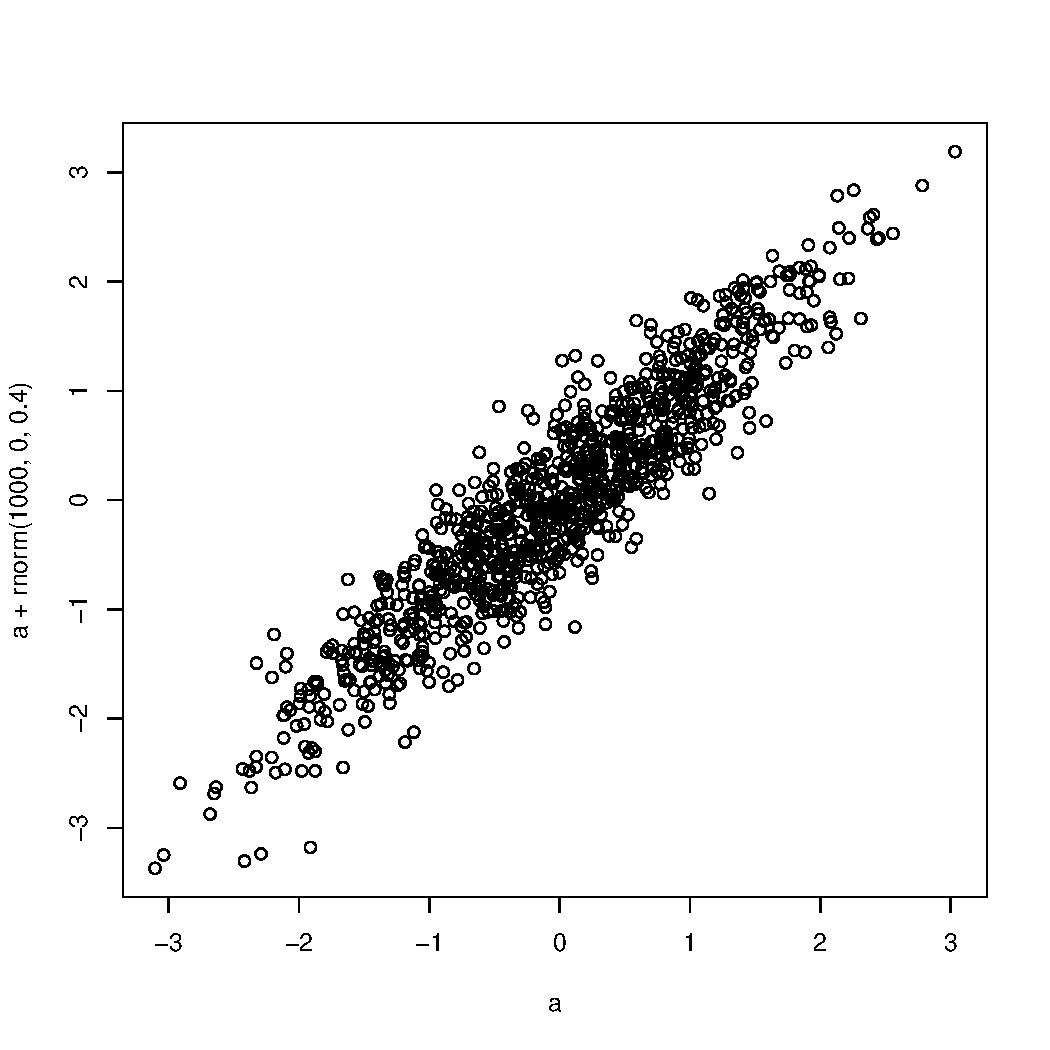
\includegraphics[width=\textwidth]{graphiques/beamer-unnamed-chunk-2-1} } 
\resizebox{!}{0.6\textheight}{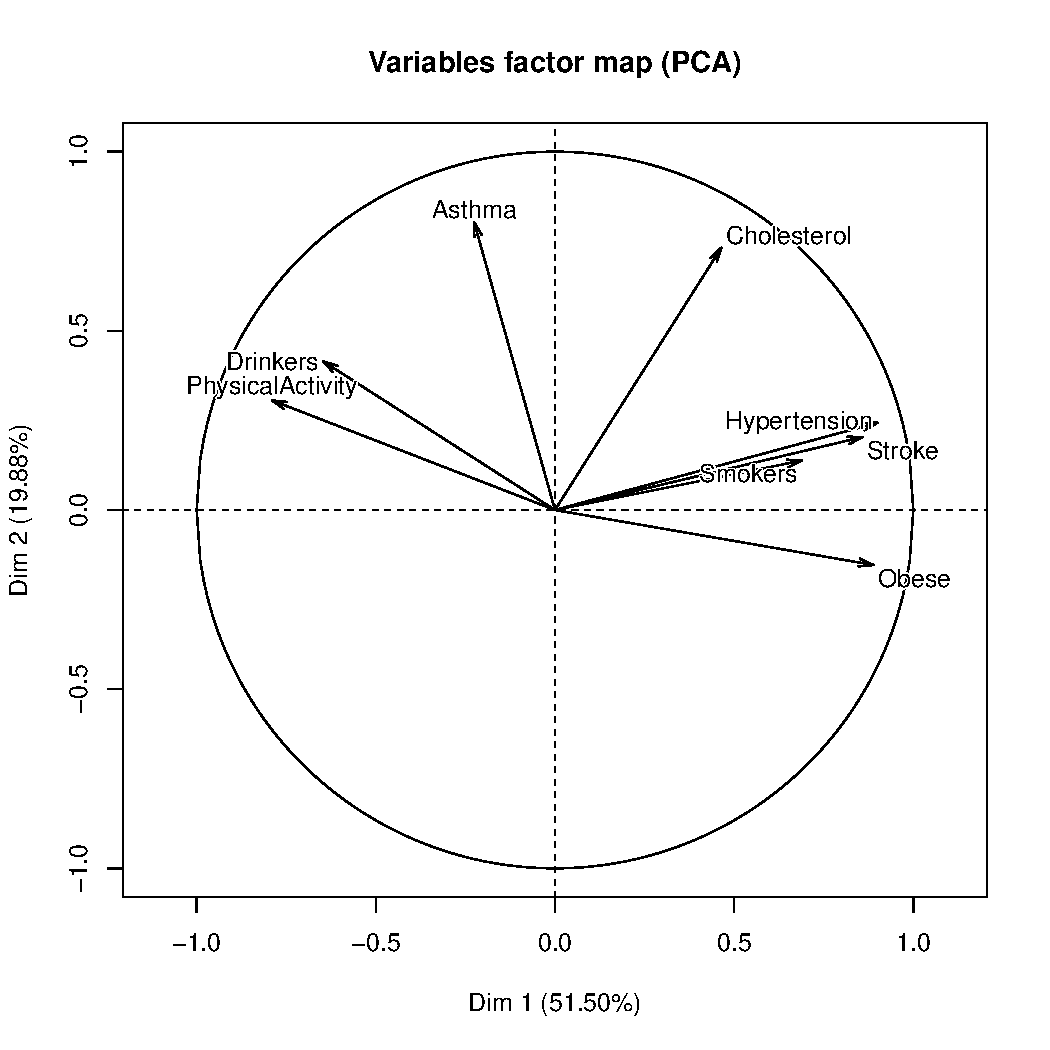
\includegraphics[width=\textwidth]{graphiques/beamer-unnamed-chunk-2-2} } 
\resizebox{!}{0.6\textheight}{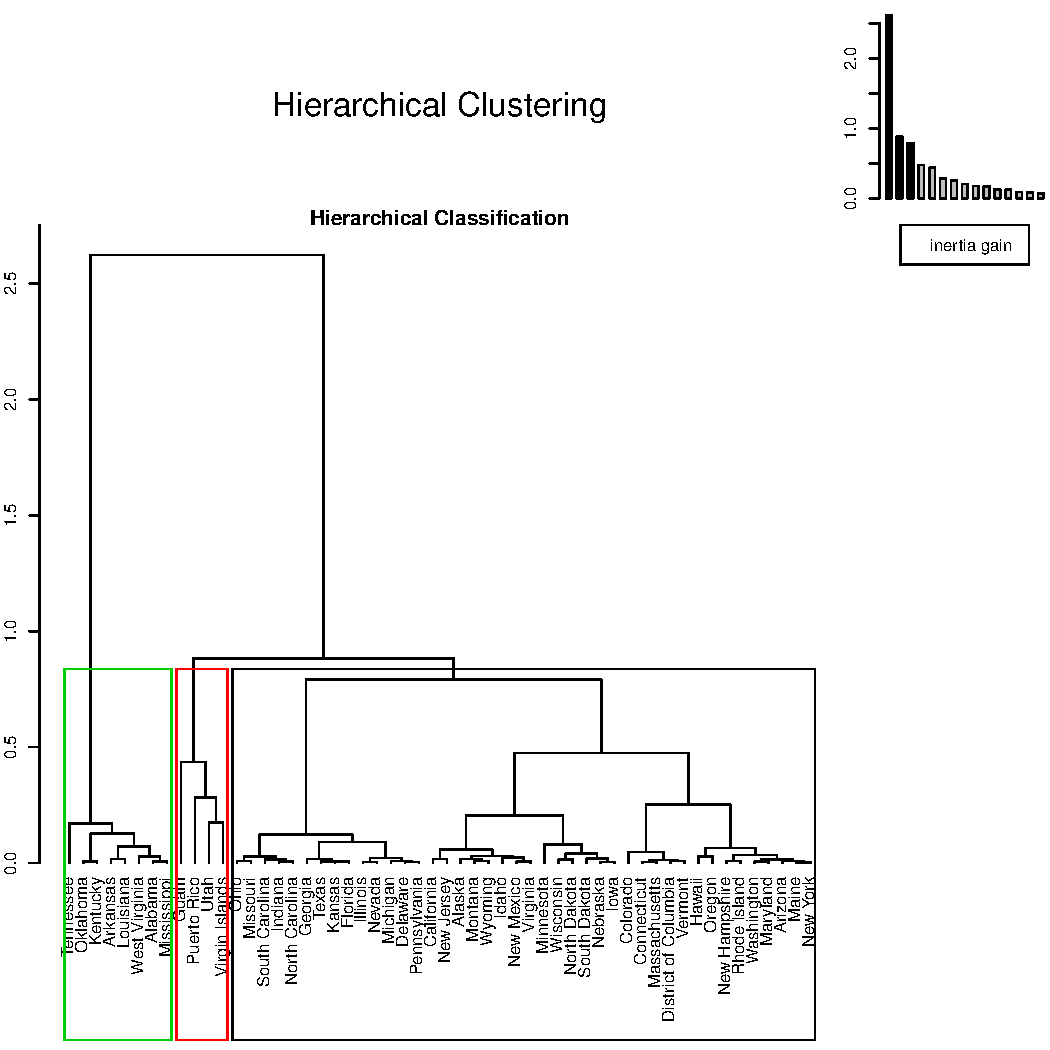
\includegraphics[width=\textwidth]{graphiques/beamer-unnamed-chunk-2-3} } 
\resizebox{!}{0.6\textheight}{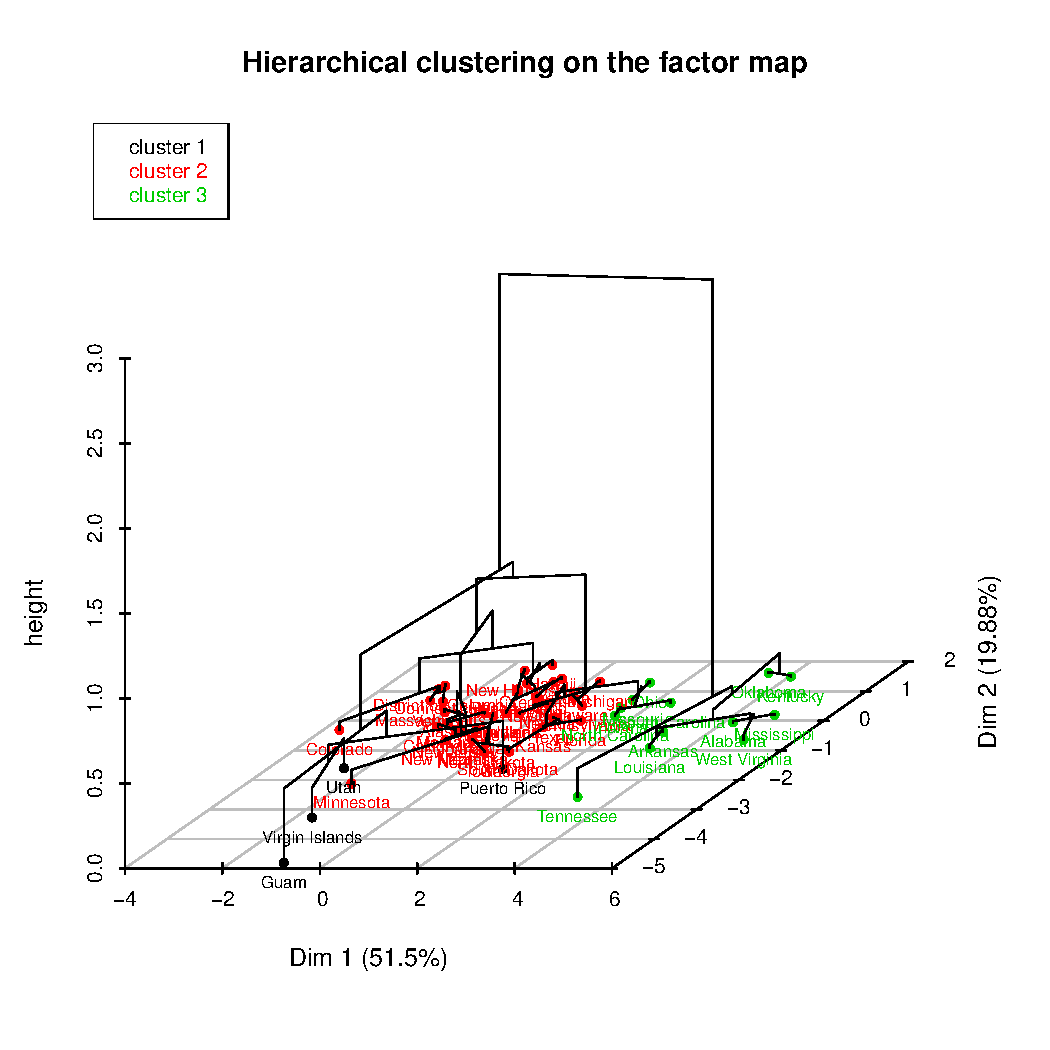
\includegraphics[width=\textwidth]{graphiques/beamer-unnamed-chunk-2-4} } 
\resizebox{!}{0.6\textheight}{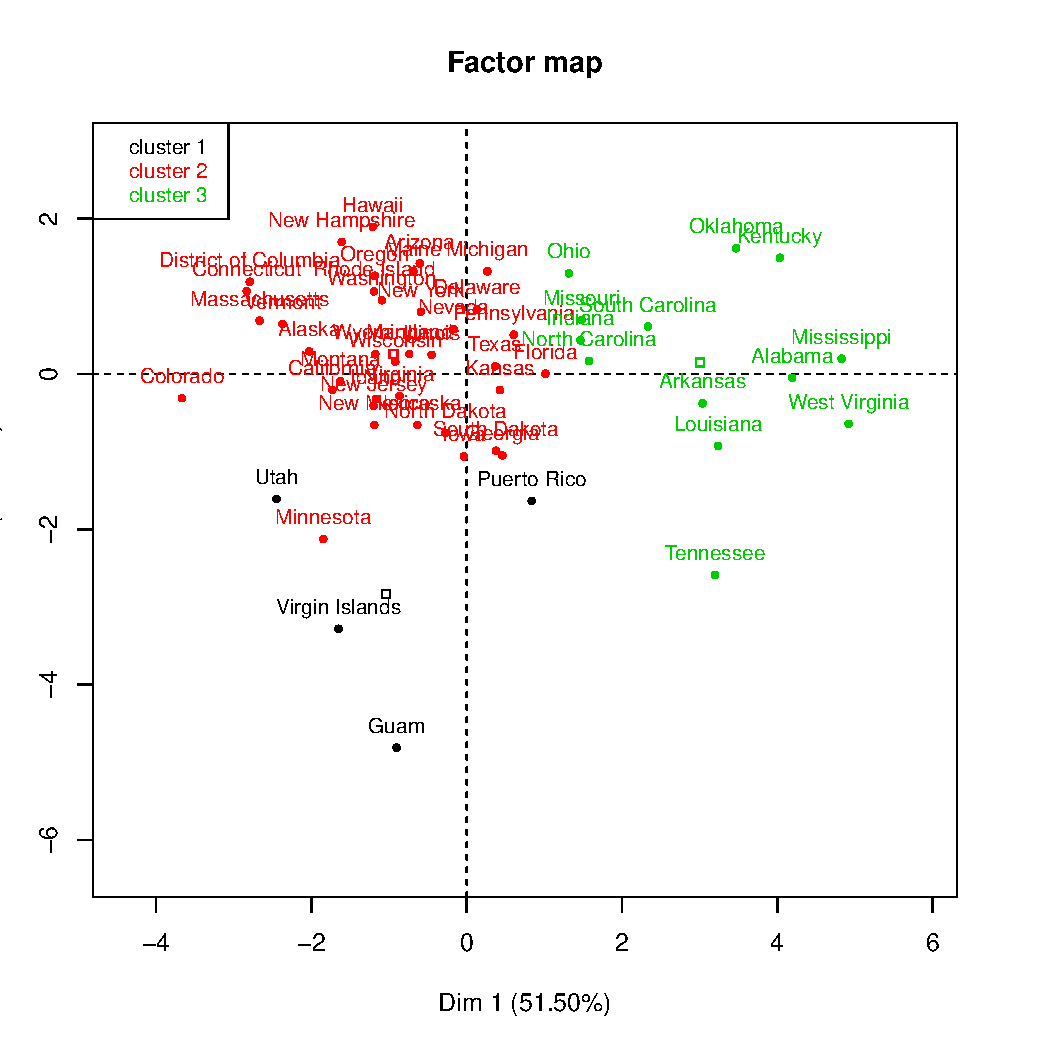
\includegraphics[width=\textwidth]{graphiques/beamer-unnamed-chunk-2-5} } 

}



\end{knitrout}

\end{document}
